\section{Scenario 2}
Barbara has moved to a new home ad now she needs for a new telephone number and an internet connection.

\begin{enumerate}
	\item She goes on \url{www.tim.it}
	\item She clicks on "Verifica la copertura 4G, Fibra e ADSL" \url{www.tim.it/verifica-copertura#tab-verifica-fisso}
	\item She enters her address information in the form and she clicks "VERIFICA". Her home is reached by fyber and adsl connection by TIM so she decides to look for a promotion. She clicks on TIM logo to return to the homepage.
	\item She overs the mouse on "OFFERTE" and clicks on "Fisso" \url{www.tim.it/offerte/fisso}
	\item She clicks on "TIM SMART FIBRA PLUS" \url{www.tim.it/offerte/fisso/internet-voce-e-timvision/fibra/tim-smart-fibra-plus}
	\item On the left side she clicks on "Costi". The costs look good so she decides to choose this promotion. Barbara clicks on "ATTIVA". The website redirects her to the ecommerce website of TIM and she continues from here.
\end{enumerate}

\subsection{Results}
\begin{enumerate}
	
%------------------------------------------------------------------------------------------------------
	
\item Report on \url{www.tim.it/verifica-copertura#tab-verifica-fisso}

\begin{center}
	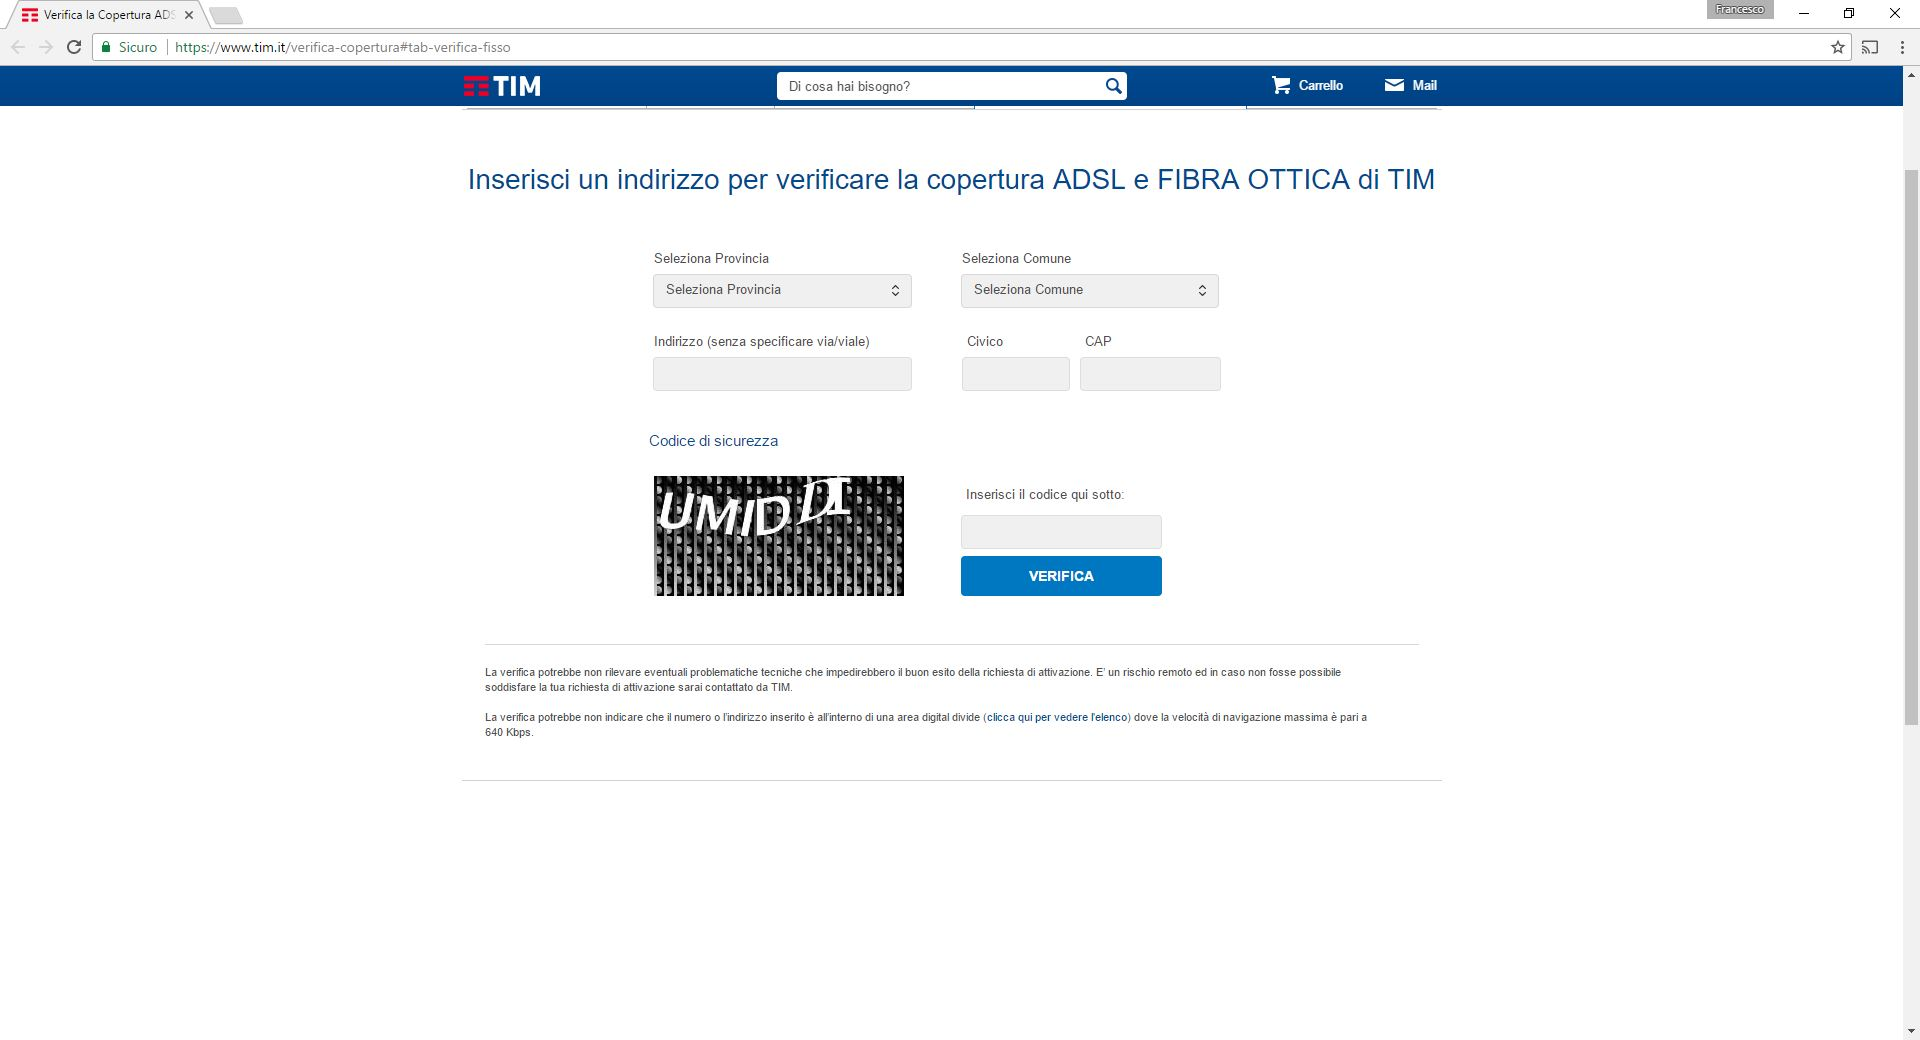
\includegraphics[width=\textwidth]{Screenshot/copertura.jpg}
\end{center}
\vspace{1cm}

	\paragraph*{Content heuristics \\ Text}
	\begin{itemize}
		\item accuracy: satisfied
		\item currency: \textcolor{red}{severely violated}\\the user cannot know if the page is updated
		\item coverage: satisfied
		\item content objectivity: n/a
		\item authority: satisfied
		\item conciseness: satisfied		
	\end{itemize}
	
	\paragraph*{General communication quality}
	\begin{itemize}
		\item text errors: satisfied
		\item multimedia consistency: satisfied
	\end{itemize}

	\paragraph*{Navigation heuristics \\ Navigation within a topic}
	\begin{itemize}
		\item segmentation: n/a
	\end{itemize}	
	
	\paragraph*{Navigation within a transition}
	\begin{itemize}
		\item transition list: n/a
	\end{itemize}
	
	\paragraph*{Navigation within a group of topics}
	\begin{itemize}
		\item introduction list: n/a
		\item group navigation: n/a
	\end{itemize}
	
	\paragraph*{Backward navigation}
	\begin{itemize}
		\item go back: \textcolor {orange}{partially violated}\\
		there isn't a "go back" functionality but the user can exploit the TIM logo to return to the homepage or select a position in the website structure path (Home $\triangleright$ Verifica copertura)
	\end{itemize}
	
	\paragraph*{Overall navigation}
	\begin{itemize}
		\item landmarks: satisfied
		\item link consistency: satisfied
		\item orientation clues: satisfied
		\item orientation clues - topic: n/a
		\item group orientation clues: n/a
		\item transition orientation clues: n/a
	\end{itemize}	
	
	\paragraph*{Visual and semantic heuristics \\ Overall graphic design }
	\begin{itemize}
		\item visual identity: satisfied\\
		the palette represents the colors of the company logo
		\item chromatic code consistency: satisfied
		\item background contrast: satisfied
		\item font size: satisfied
		\item font colour: satisfied
		\item font type: satisfied
		\item anchor identity: satisfied
		\item anchor states: satisfied
		\item icon consistency: satisfied
	\end{itemize}
	
	\paragraph*{Page layout}
	\begin{itemize}
		\item visual proximity: satisfied
		\item layout conventions: satisfied
		\item semiotics: satisfied
	\end{itemize}	
	
	\paragraph*{Cognitive heuristics \\ Single page}
	\begin{itemize}
		\item information overload: satisfied
	\end{itemize}	
	
	\paragraph*{Information architecture}
	\begin{itemize}
		\item classification adequacy within group of topics: satisfied
		\item website mental map: satisfied
	\end{itemize}

%------------------------------------------------------------------------------------------------------

\item Report on \url{www.tim.it/offerte/fisso}

\begin{center}
	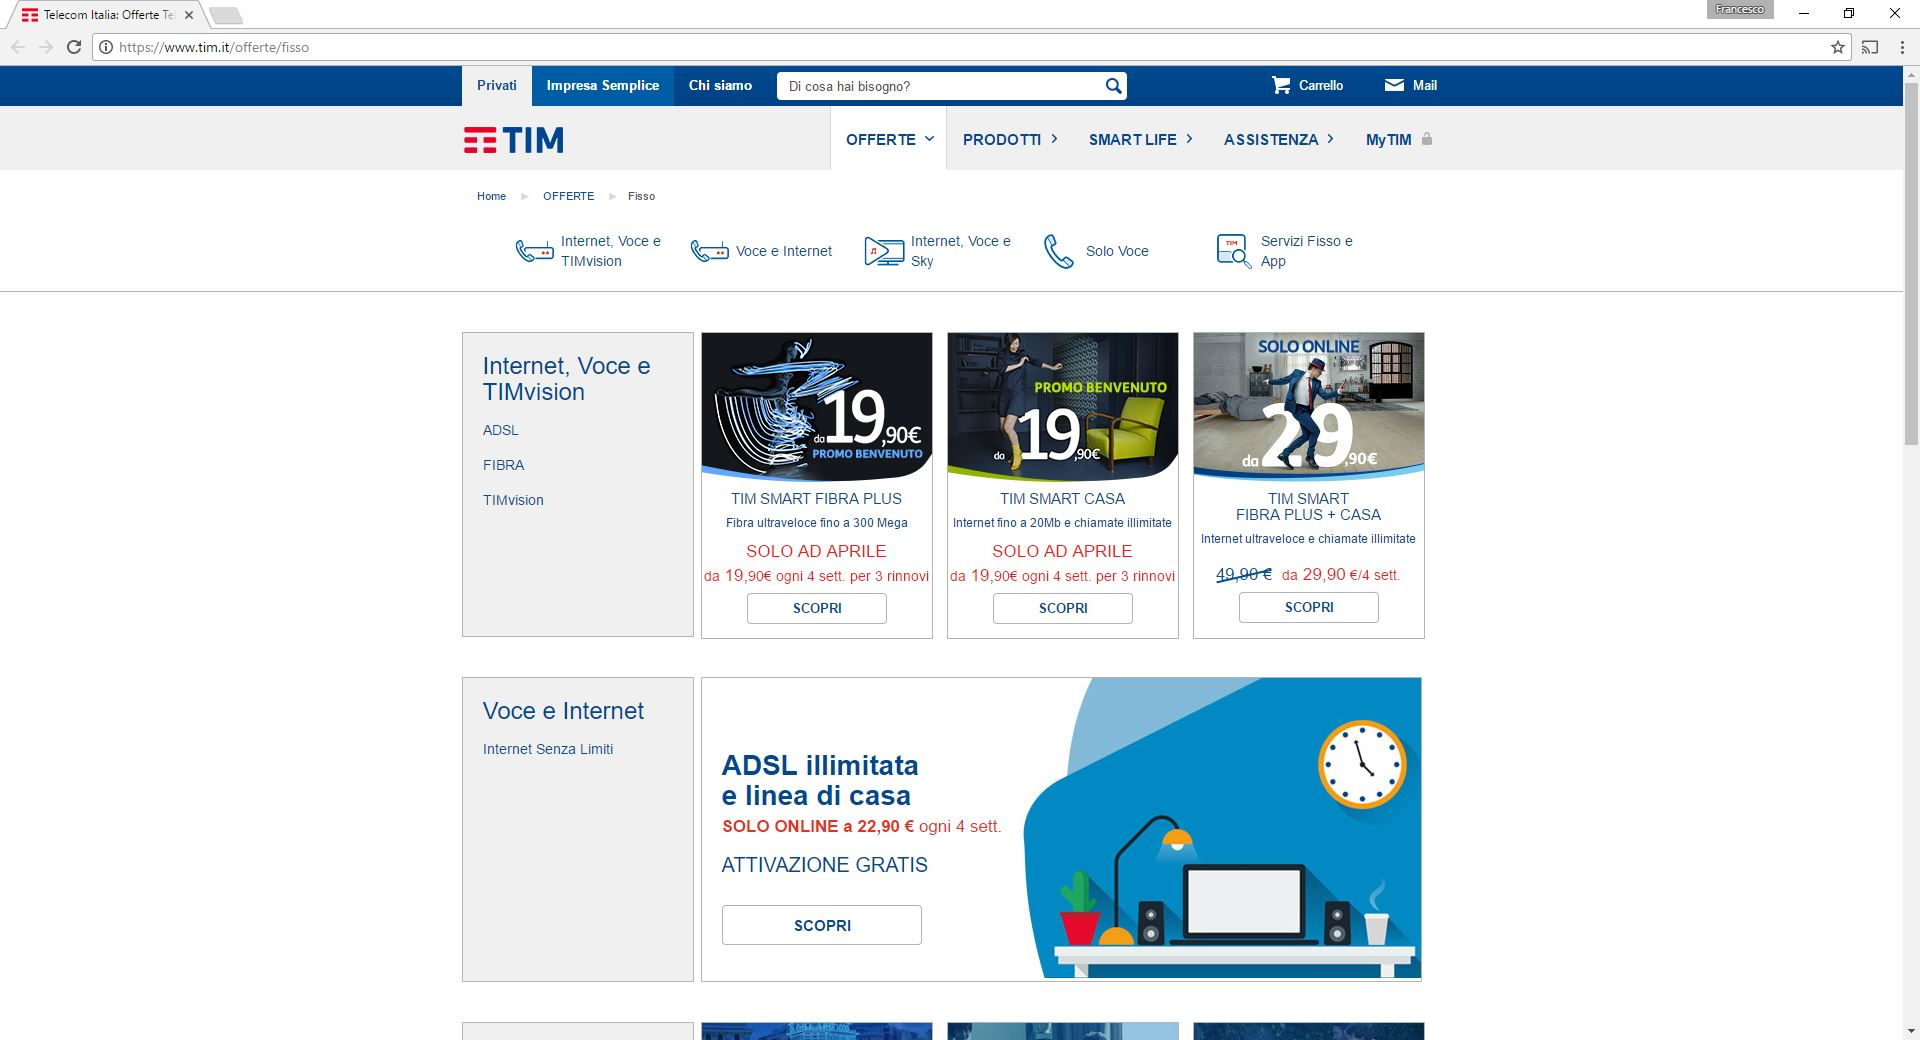
\includegraphics[width=\textwidth]{Screenshot/fisso.jpg}
\end{center}
\vspace{1cm}

	\paragraph*{Content heuristics \\ Text}
	\begin{itemize}
		\item accuracy: satisfied
		\item currency: \textcolor{orange}{partially violated}\\
		the user knows that the site is updated through the promotions that are limited for the current period
		\item coverage: satisfied
		\item content objectivity: n/a
		\item authority: satisfied
		\item conciseness: satisfied		
	\end{itemize}

	\paragraph*{General communication quality}
	\begin{itemize}
		\item text errors: satisfied
		\item multimedia consistency: satisfied
	\end{itemize}

	\paragraph*{Navigation heuristics \\ Navigation within a topic}
	\begin{itemize}
		\item segmentation: n/a
	\end{itemize}	
	
	\paragraph*{Navigation within a transition}
	\begin{itemize}
		\item transition list: n/a
	\end{itemize}
	
	\paragraph*{Navigation within a group of topics}
	\begin{itemize}
		\item introduction list: satisfied
		\item group navigation: satisfied
	\end{itemize}

	\paragraph*{Backward navigation}
	\begin{itemize}
		\item go back: \textcolor {orange}{partially violated}\\
		there isn't a "go back" functionality but the user can exploit the TIM logo to return to the homepage or select a position in the website structure path (Home $\triangleright$ OFFERTE $\triangleright$ Fisso)
	\end{itemize}
	
	\paragraph*{Overall navigation}
	\begin{itemize}
		\item landmarks: satisfied
		\item link consistency: satisfied
		\item orientation clues: satisfied
		\item orientation clues - topic: n/a
		\item group orientation clues: satisfied
		\item transition orientation clues: n/a
	\end{itemize}	
	
	\paragraph*{Visual and semantic heuristics \\ Overall graphic design }
	\begin{itemize}
		\item visual identity: satisfied
		\item chromatic code consistency: satisfied
		\item background contrast:satisfied
		\item font size: satisfied
		\item font colour: satisfied
		\item font type: satisfied
		\item anchor identity: satisfied
		\item anchor states: satisfied
		\item icon consistency: satisfied
	\end{itemize}
	
	\paragraph*{Page layout}
	\begin{itemize}
		\item visual proximity: satisfied
		\item layout conventions: satisfied
		\item semiotics: satisfied
	\end{itemize}	
	
	\paragraph*{Cognitive heuristics \\ Single page}
	\begin{itemize}
		\item information overload: satisfied
	\end{itemize}	
	
	\paragraph*{Information architecture}
	\begin{itemize}
		\item classification adequacy within group of topics: satisfied
		\item website mental map: satisfied
	\end{itemize}
\newpage

%------------------------------------------------------------------------------------------------------

\item Report on \url{www.tim.it/offerte/fisso/internet-voce-e-timvision/fibra/tim-smart-fibra-plus}

\begin{center}
	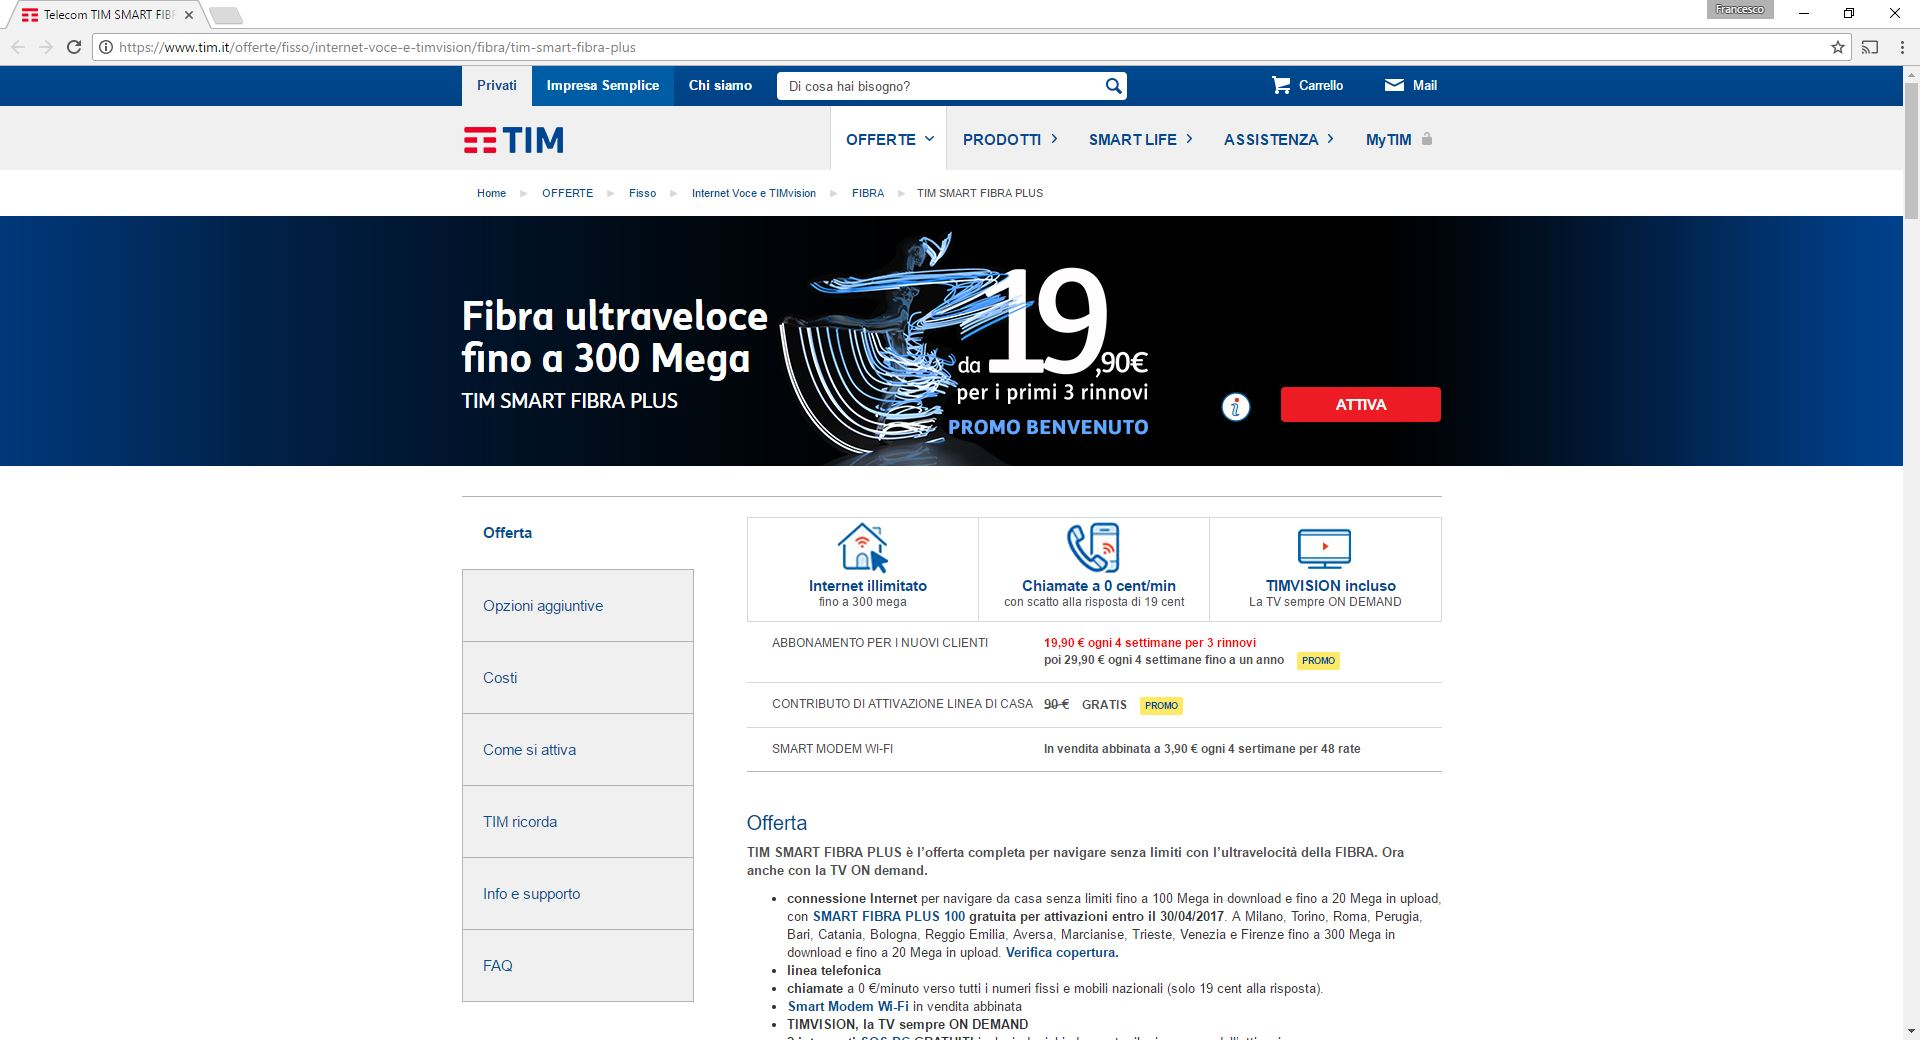
\includegraphics[width=\textwidth]{Screenshot/fibra.jpg}
\end{center}
\vspace{1cm}

	\paragraph*{Content heuristics \\ Text}
	\begin{itemize}
		\item accuracy: satisfied
		\item currency:  \textcolor{orange}{partially violated}\\
		the user knows that the site is updated through the promotions that are limited for the current period
		\item coverage: satisfied
		\item content objectivity: satisfied
		\item authority: satisfied
		\item conciseness: satisfied		
	\end{itemize}

	\paragraph*{General communication quality}
	\begin{itemize}
		\item text errors: satisfied
		\item multimedia consistency: satisfied
	\end{itemize}

	\paragraph*{Navigation heuristics \\ Navigation within a topic}
	\begin{itemize}
		\item segmentation: satisfied\\
		the information of the topic are organized in sub-sections (accessible on the left side) on the same page
	\end{itemize}	

	\paragraph*{Navigation within a transition}
	\begin{itemize}
		\item transition list: satisfied
	\end{itemize}

	\paragraph*{Navigation within a group of topics}
	\begin{itemize}
		\item introduction list: n/a
		\item group navigation: n/a
	\end{itemize}

	\paragraph*{Backward navigation}
	\begin{itemize}
		\item go back: \textcolor {orange}{partially violated}\\
		there isn't a "go back" functionality but the user can exploit the TIM logo to return to the homepage or select a position in the website structure path (Home $\triangleright$ OFFERTE $\triangleright$ Fisso $\triangleright$ Internet Voce e TIMvision $\triangleright$ Fibra $\triangleright$ TIM SMART FIBRA PLUS)
	\end{itemize}

	\paragraph*{Overall navigation}
	\begin{itemize}
		\item landmarks: satisfied
		\item link consistency: satisfied
		\item orientation clues: satisfied
		\item orientation clues - topic: satisfied
		\item group orientation clues: satisfied
		\item transition orientation clues: satisfied
	\end{itemize}	

	\paragraph*{Visual and semantic heuristics \\ Overall graphic design }
	\begin{itemize}
		\item visual identity: satisfied (the colors represents the logo of the company)
		\item chromatic code consistency: satisfied
		\item background contrast:satisfied
		\item font size: satisfied
		\item font colour: satisfied
		\item font type: satisfied
		\item anchor identity: satisfied
		\item anchor states: satisfied
		\item icon consistency: satisfied
	\end{itemize}

	\paragraph*{Page layout}
	\begin{itemize}
		\item visual proximity: satisfied
		\item layout conventions: satisfied
		\item semiotics: satisfied
	\end{itemize}

	\paragraph*{Cognitive heuristics \\ Single page}
	\begin{itemize}
		\item information overload: satisfied
	\end{itemize}	

	\paragraph*{Information architecture}
	\begin{itemize}
		\item classification adequacy within group of topics: satisfied
		\item website mental map: satisfied
	\end{itemize}
	\end{enumerate}